\chapter{Requirements}
\label{requirements}

\section{Introduction}

In eliciting possible requirements for the site, there was a discussion with three club members with varying backgrounds and experience within the club.

\begin{table}[H]
\caption{Stakeholders for Requirements Elicitation}
\begin{center}
    \begin{tabular}{ | l | l | l | l | l| p{5cm} |}
    \hline
    Name & Age Bracket & Club Role & Club Membership & Work Background \\ \hline
	'Larry' & 35 - 45& Committee Member & 5 years & Senior Software Engineer \\ \hline
	'Moe' & 18 - 25 & New Member & 1 year & Graduate Software Engineer \\ \hline
	'Curly' & 55+ & Senior Member & 10+ years & Retired Public Servant \\ \hline
    \end{tabular}
\end{center}
\label{fig:userelicit}
\end{table}



\begin{table}[H]
\begin{enumerate}
\item Book Court
\begin{itemize}
\item Allow user to book a slot on a timetable for a court
\end{itemize}
\item Remove Booking
\begin{itemize}
\item Allow user to book a slot on a timetable for a court
\end{itemize}
\item Register for Tournament
\begin{itemize}
\item Allow users to register for a tournament
\end{itemize}
\item Contact Members
\begin{itemize}
\item Easy way to contact all members
\end{itemize}
\item Member Directory
\begin{itemize}
\item A list of all members, contact details, roles
\end{itemize}
\item News Section
\begin{itemize}
\item Create new items to display for members
\end{itemize}
\item Members Area
\begin{itemize}
\item A secure area that only members could access
\end{itemize}
\item Member Application
\begin{itemize}
\item Automated registration, replace old paper form
\end{itemize}
\item Club Map
\begin{itemize}
\item Directions to the club for new members and non-local visitors
\end{itemize}
\item Contact Details
\begin{itemize}
\item Information on how to contact within the club for specific needs
\end{itemize}
\item Statistics
\begin{itemize}
\item Such as games played, Win/Loss ratio
\end{itemize}


\end{enumerate}
\label{fig:secRoles}
\end{table}
Table ~\ref{fig:reqbreakdown} refers to each numbered requirement, and whether it was brought up by a stakeholder during the elicitation process.
\begin{table}[H]
\caption{Requested Feature Breakdown}
\begin{center}
    \begin{tabular}{ | l | l | l | l | l| l| l| l| l| l|l| p{.22cm} |}
    \hline
     \textit{Name}& 1& 2 & 3 & 4 & 5 & 6 & 7 & 8 & 9 & 10 & 11\\ \hline
	 'Larry' & N & N & Y & Y & Y & N & Y & Y & Y & Y & N\\ \hline
	  'Moe' & Y & Y & Y & Y & N & N & N & N & N & N & Y\\ \hline
	    'Curly' & Y & Y & N & N & N & N & N & Y & Y & N & N\\ \hline
    \end{tabular}
\end{center}
\label{fig:reqbreakdown}
\end{table}
\section{Method for Requirements}

\subsection{Storyboarding}

At an early stage of the application, rough storyboards were prepared for the FYP presentation. These storyboards were used to demonstrate how a page, such as the timetable shown in Figure~\ref{fig:timetableSB}, would be displayed by the application.

\begin{figure}[H]
\begin{center}
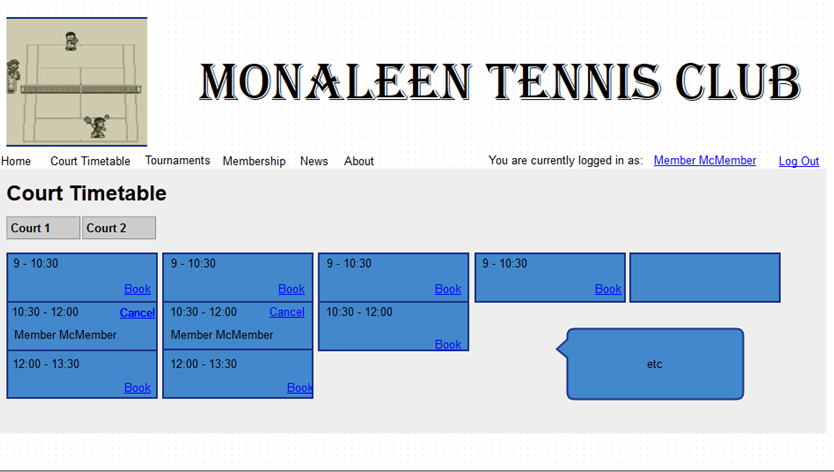
\includegraphics[width=14cm]{storyboard.png}
\end{center}
\caption{Timetable Storyboard, October 2013}
\label{fig:timetableSB}
\end{figure}

The storyboarding visualised aspects of the site, and gave a rough idea of functionality that would be needed within the application. 

\section{Application}

\section{Functional Requirements}

\subsection{User} 

There are a number of actions that a user needs to be able to accomplish within the system. The user should be able to register their details within the system to create an account. Once the account is created, the user should be able to impact other site features, such as the timetable, based on their authority within the application. 

\begin{enumerate}
\item Register
\item Login
\item Register for a tournament
\item View members registered for a tournament
\item View all member contact details
\item Book a slot on timetable
\item Remove a booking that they placed on a timetable
\item Report a no show for a booked slot
\end{enumerate}

\subsection{Timetable}

The timetable is the core aspect of the application, and one that would be most likely to be used by all members, not just those involved competitively. While the regular member would only be concerned with the booking of slots, there are a number of requirements defined for use by the administrator in order to configure a relevant timetable not the club. The timetable needs to be flexible to allow the administrator full control at all stages.

\begin{enumerate}
\item Flexible 
\item Edit individual slots
\item Define a template for a timetable
\item Reset timetable
\item Define look ahead for timetable (how many weeks in advance a user can see)
\item Book a slot on timetable
\item Remove a booking that they placed on a timetable
\item Report a no show for a booked slot
\end{enumerate}

\subsection{Tournament}

\subsection{Timetable}

\section{Use Cases}

\begin{figure}[H]
\begin{center}
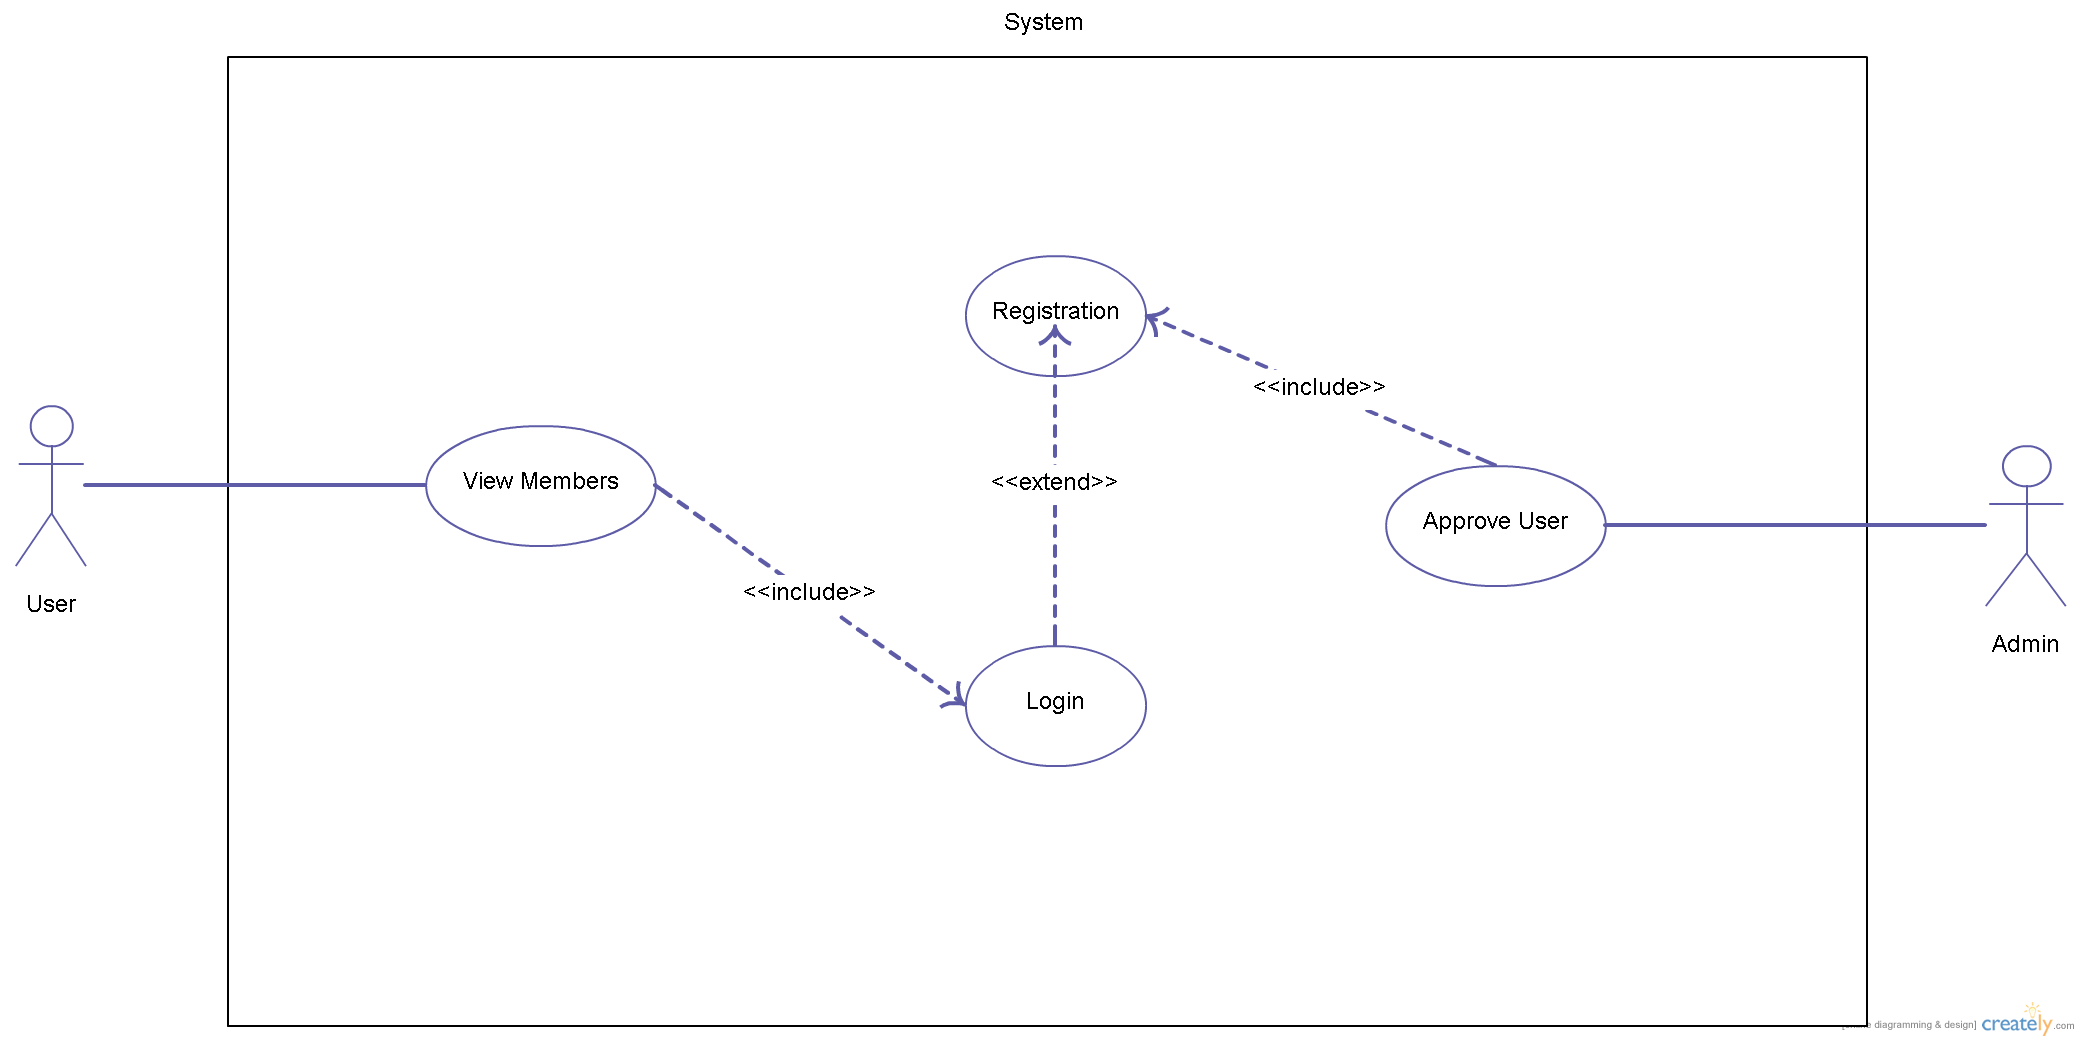
\includegraphics[width=14cm]{usecaselogin.png}
\end{center}
\caption{Use case for User login}
\label{fig:usecaselogin}
\end{figure}

\begin{usecase}

\addtitle{Use Case 1}{View All Members} 

%Scope: the system under design
\addfield{Scope:}{System-wide}

%Level: "user-goal" or "subfunction"
\addfield{Level:}{User can view a list of all registered, and approved, members of the club}

%Primary Actor: Calls on the system to deliver its services.
\addfield{Primary Actor:}{All Registered and Authenticated Users}

%Stakeholders and Interests: Who cares about this use case and what do they want?
\additemizedfield{Stakeholders and Interests:}{
	\item All Users: contact information for club members
}

%Preconditions: What must be true on start and worth telling the reader?
\addfield{Preconditions:}{User is registered and approved}
%when multiple
%\additemizedfield{Preconditions:}{} 

%Postconditions: What must be true on successful completion and worth telling the reader
\addfield{Postconditions:}{User must be authenticated by the framework}
%when multiple
%\additemizedfield{Preconditions:}{}

%Main Success Scenario: A typical, unconditional happy path scenario of success.
\addscenario{Main Success Scenario:}{
	\item User logs in
	\item User clicks on View Members
	\item System displays member information
}

%Extensions: Alternate scenarios of success or failure.
\addscenario{Extensions:}{
	\item[1.a] Invalid login data:
		\begin{enumerate}
		\item[1.] System shows failure message
		\item[2.] User returns to step 1
		\end{enumerate}
	\item[1.a] User not approved:
		\begin{enumerate}
		\item[1.] System shows failure message
		\item[2.] Admin is emailed about attempted access by unapproved member
		\end{enumerate}
}

%Frequency of Occurrence: Influences investigation, testing and timing of implementation.
\addfield{Frequency of Occurrence:}{High}

\end{usecase}

\section{Non Functional Requirements}

\subsection{Security}

\subsection{Extensibility}

\subsection{Usability}
